\documentclass[a4paper,11pt,dvipdfmx]{jsarticle}

\usepackage{bm}
\usepackage[dvipdfmx]{graphicx}
\usepackage[dvipdfmx]{color}
\usepackage{ascmac}
\usepackage{amsmath}
\usepackage{amssymb}
\usepackage{siunitx}
\usepackage{otf}
\usepackage[dvipdfmx]{graphicx}
\pagestyle{plain}
\usepackage{float}
\usepackage[dvipdfmx]{hyperref}
\usepackage{pxjahyper}
\usepackage{here}
\usepackage{titlesec}
\titleformat*{\section}{\LARGE\bfseries}
\titleformat*{\subsection}{\normalsize\bfseries}
\usepackage{url}
\usepackage[table,xcdraw]{xcolor}
\hypersetup{% hyperrefオプションリスト
setpagesize=false,
 bookmarksnumbered=true,%
 bookmarksopen=true,%
 colorlinks=true,%
 linkcolor=blue,
 citecolor=blue,
}

\begin{document}
\setcounter{page}{1}
\renewcommand\thefootnote{\arabic{footnote})}
\subsection{微分散乱断面積の理論}
本節では今回の散乱実験で重要な物理量となる微分散乱断面積について考える。
ここでは微分散乱断面積を重心系における散乱角$\theta$で定義する。
\subsubsection{異なる2粒子系におけるCoulomb散乱\cite{2017}\cite{ion}}
加速された陽子がターゲットに入射して散乱する主な原因としてCoulomb力による散乱(Rutherford散乱)が考えられる。本節では異なる2粒子系についてRutherford散乱がどのように表されるかを量子論的に考える。

今、中心力が働く場に対する入射粒子の相対運動を考え、入射粒子を平面波、散乱粒子を球状波で表し、図\ref{fig:qmscattering}のように座標を取る。また、異なる2粒子の原子番号を$Z_{1}$,$Z_{2}$とする。
\begin{figure}[hbtp]
\centering
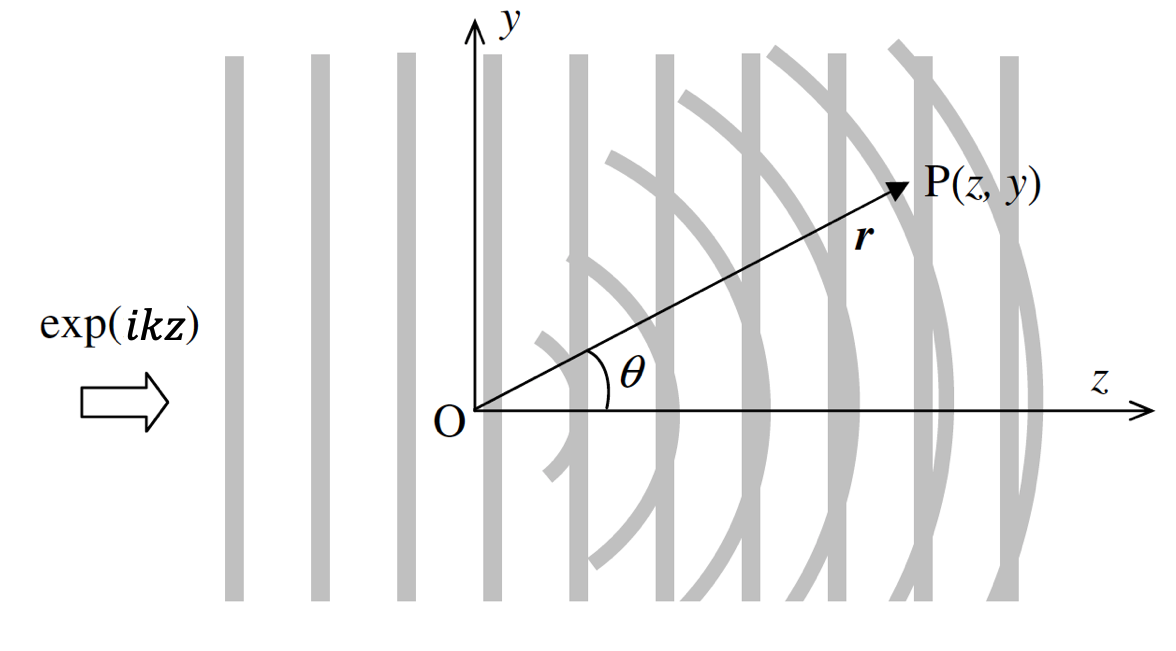
\includegraphics[width=10cm]{picture/cstheory/qmscattering.png}
\caption{散乱角$\theta$、入射方向$z$の散乱の様子(\cite{ion}より引用し、一部改変)}
\label{fig:qmscattering}
\end{figure}

クーロン相互作用している2粒子系のSchrödinger方程式はCoulombポテンシャル
\begin{equation*}
    V(r)=\frac{Z_{1}Z_{2}e^{2}}{4\pi\varepsilon_{0}r} 
\end{equation*}
を用いて
\begin{equation}
\left(-\frac{\hbar^{2}}{2m}\Delta + \frac{Z_{1}Z_{2}e^{2}}{4\pi\varepsilon_{0}r}\right)\Psi =E\Psi
\label{eq:sch}
\end{equation}
のように書くことができる。ここで、
\begin{equation}
E=\frac{\hbar^{2}k^{2}}{2m}=\frac{1}{2}mv^{2}
\end{equation}
は重心系における運動エネルギーである。極座標から放物線座標への変換式
\begin{gather*}     
      \xi\,=\, r - z \,=\, r\left(1 - \cos\theta\right), \\  
      \eta\,=\, r + z \,=\, r\left(1 + \cos\theta\right), \\
      \psi\,=\,\psi. 
\end{gather*}
を用いて式\eqref{eq:sch}を変換すると、
\begin{equation}
-\frac{\hbar^{2}}{2m}\frac{4}{\xi+\eta}\left[\frac{\partial}{\partial\xi}\left(\xi\frac{\partial\Psi}{\partial\xi}\right)+ \frac{\partial}{\partial\eta}\left(\eta\frac{\partial\Psi}{\partial\eta}\right)\right]+ \frac{Z_{1}Z_{2}e^{2}}{2\pi\varepsilon_{0}\left(\xi+\eta\right)}\Psi =E\Psi
\label{eq:sch2}
\end{equation}
となる。

ここで$\Psi$を
\begin{equation}
    \Psi = \exp(ikz)\chi\left(r,\theta\right)=  \exp\left[-ik\left(\xi-\eta\right)/2\right]\chi\left(\xi,\eta\right)
    \label{eq:Psi}
\end{equation}
とする。

今、$\Psi$は遠方では外向きの球状波に漸近すべきなので、式\eqref{eq:Psi}より、$\chi$は遠方で \\*\:$\exp[ik(r-z)] \,=\,\exp(ik\xi)$\,という項に比例するはずである。ところで、式\eqref{eq:sch2}より$\Psi$は$\xi$と$\eta$を交換しても不変なので、$\chi$が変数$\eta$を含むとすれば、$\chi$は遠方では $\exp(ik\eta) \,=\,\exp[(ik(r+z)]$\, \\
という項に比例することになる。しかし、これは逆向きの入射波に相当するものであり、 \\
不適切である。よって、$\chi$は$\eta$を含まない。

式\eqref{eq:Psi}を式\eqref{eq:sch2}に代入し、$\chi$が$\xi$のみの関数であることを考慮して、
\begin{equation}
    \xi\frac{d^{2}\chi}{d\xi^{2}} + \left(1 - ik\xi\right)\frac{d\chi}{d\xi} -\frac{\kappa k}{2}\chi = 0
    \label{eq:tyokika}
\end{equation}
を得る。ここで
\begin{gather*}
\kappa = \frac{Z_{1}Z_{2}e^{2}}{2\pi\varepsilon_{0}\hbar v}
\end{gather*}
であり、BohrのCoulomb散乱パラメータと呼ばれる無次元数である。\footnote{$\dfrac{\kappa}{2}$をBohrのCoulomb散乱パラメータと呼ぶ流儀もある。}

この解を求めるために合流型超幾何関数を考える。一般に$A$,$B$を定数として
\begin{equation}
        X\frac{d^{2}F}{dX^{2}} + \left(B - X\right)\frac{dF}{dX} -AF = 0
        \label{eq:tyo}
\end{equation}
の解$F$を合流型超幾何関数と呼ぶ。$X=0$で正則なものの解は、
\begin{align} 
     F(A,B,X) &= \sum_{j=0}^{\infty}\frac{\Gamma\left(A+j\right)\Gamma\left(B\right)X^{j}}{\Gamma\left(A\right)\Gamma\left(B+j\right)\Gamma\left(1+j\right)} \notag\\
    &= 1+ \frac{A}{B1!}X+\frac{A\left(A+1\right)}{B\left(B+1\right)2!}X^{2}+\frac{A\left(A+1\right)\left(A+2\right)}{B\left(B+1\right)\left(B+2\right)3!}X^{3}+\cdots 
    \label{eq:tyokika2}
  \end{align}

と表される。$\Gamma$はRe$(z)>0$の時
\begin{equation*}
    \Gamma(z)= \int_{0}^{\infty}e^{-t}t^{z-1}dt
\end{equation*}
で定義される$\Gamma$関数である。

式\eqref{eq:tyokika}を
\begin{equation*}
   ik\xi\frac{d^{2}\chi}{d\left(ik\xi\right)^{2}} + \left(1 - ik\xi\right)\frac{d\chi}{d\left(ik\xi\right)} -\frac{-i\kappa}{2}\chi = 0 
\end{equation*}
と変形し、\eqref{eq:tyo}と比較すると、解$\chi$は
\begin{displaymath}
\chi=F\left(\frac{-i\kappa}{2},\,1,\,ik\xi\right)
\end{displaymath}
となる。規格化した式\eqref{eq:sch}の解は、
\begin{align}
     \Psi \,&=\, \exp\left(-\frac{\pi\kappa}{4}+ikz\right)\Gamma\left(1+\frac{i\kappa}{2}\right)F\left(\frac{-i\kappa}{2},\,1,\,ik\xi\right) \notag\\
     &= \,\exp\left(-\frac{\pi\kappa}{4}+ikr\cos\theta\right)\Gamma\left(1+\frac{i\kappa}{2}\right)F\left(\frac{-i\kappa}{2},\,1,\,2ikr\sin^2\frac{\theta}{2}\right) \notag\\
     &= \,\left(1 - \frac{i\kappa^{2}}{8kr\sin^2\frac{\theta}{2}}\right)\exp\left(i[kr\cos\theta+\frac{\kappa}{2}\ln(2kr\sin^2\frac{\theta}{2})]\right) \notag\\
     &+ \,\frac{\kappa}{4kr\sin^2\frac{\theta}{2}}\exp\left(i[kr-\frac{\kappa}{2}\ln(2kr\sin^2\frac{\theta}{2})+\pi+2\eta_{0}]\right)\label{eq:kikakukai}
\end{align}
と表される。ただし、2行目から3行目の変形の際、$kr\gg1$,すなわち入射粒子のde  Broglie波長$(2\pi/k)$に比べて$r$が十分大きいとした。また、$\exp(2i\eta_{0})=\Gamma(1+i\kappa/2)/\Gamma(1-i\kappa/2)$である。

式\eqref{eq:kikakukai}の第一項は透過波、第二項は散乱波とみなせる。$kr\rightarrow \infty$とすると、\\*
$\Psi = \exp(ikr\cos\theta)  =\exp(ikz)$、つまり第一項の入射(透過)波のみとなって、散乱波は無視されてしまうことに注意する。遠方では、$kr\gg\ln{kr}$なので式\eqref{eq:kikakukai}の漸近形は
\begin{equation}
 \Psi \sim \exp(ikz)+f(\theta)\,\frac{\exp(ikr)}{r} 
 \label{eq:zenkinn}
\end{equation}
のようになる。このとき、$\kappa$と$k$を戻して係数比較すれば、
\begin{equation}
    f(\theta)=\frac{Z_{1}Z_{2}e^2}{8\pi\varepsilon_{0}mv^2}\exp\left(i[-\frac{\kappa}{2}\ln(2kr\sin^2\frac{\theta}{2})+\pi+2\eta_{0}]\right)\frac{1}{\sin^2\frac{\theta}{2}}
    \label{eq:sanransinpuku}
\end{equation}
となり、この式\eqref{eq:sanransinpuku}はCoulomb散乱の散乱振幅と呼ばれる。
微分散乱断面積は散乱振幅の絶対値の2乗で表されるので、
\begin{align}
    \frac{d\sigma}{d\Omega} = |f(\theta)|^{2}=\left(\frac{Z_{1}Z_{2}e^2}{8\pi\varepsilon_{0}mv^2}\right)^{2}\frac{1}{\sin^4\frac{\theta}{2}} \notag\\
    = \left(\frac{Z_{1}Z_{2}e^2}{16\pi\varepsilon_{0}E}\right)^{2}\frac{1}{\sin^4\frac{\theta}{2}}\label{eq:Rutherford}
\end{align}
式\eqref{eq:Rutherford}をRutherfordの散乱公式という。

今回の実験では陽子を入射させるので、Rutherfordの散乱公式は以下のように書ける。
\begin{equation}
    \frac{d\sigma}{d\Omega}=\left(\frac{Ze^2}{16\pi\varepsilon_{0}E}\right)^{2}\frac{1}{\sin^4\frac{\theta}{2}}\label{eq:Ruther}
\end{equation}
$Z$はターゲットの原子番号、$E$は入射粒子のエネルギー、$\theta$は重心系における散乱角である。
\eqref{eq:Ruther}を今回の実験で用いる標的ごとにグラフに表すと図\ref{fig:cross}のようになる。
($E=$\;3\;MeV) 
\\
\\
\begin{figure}[htbp]
\centering
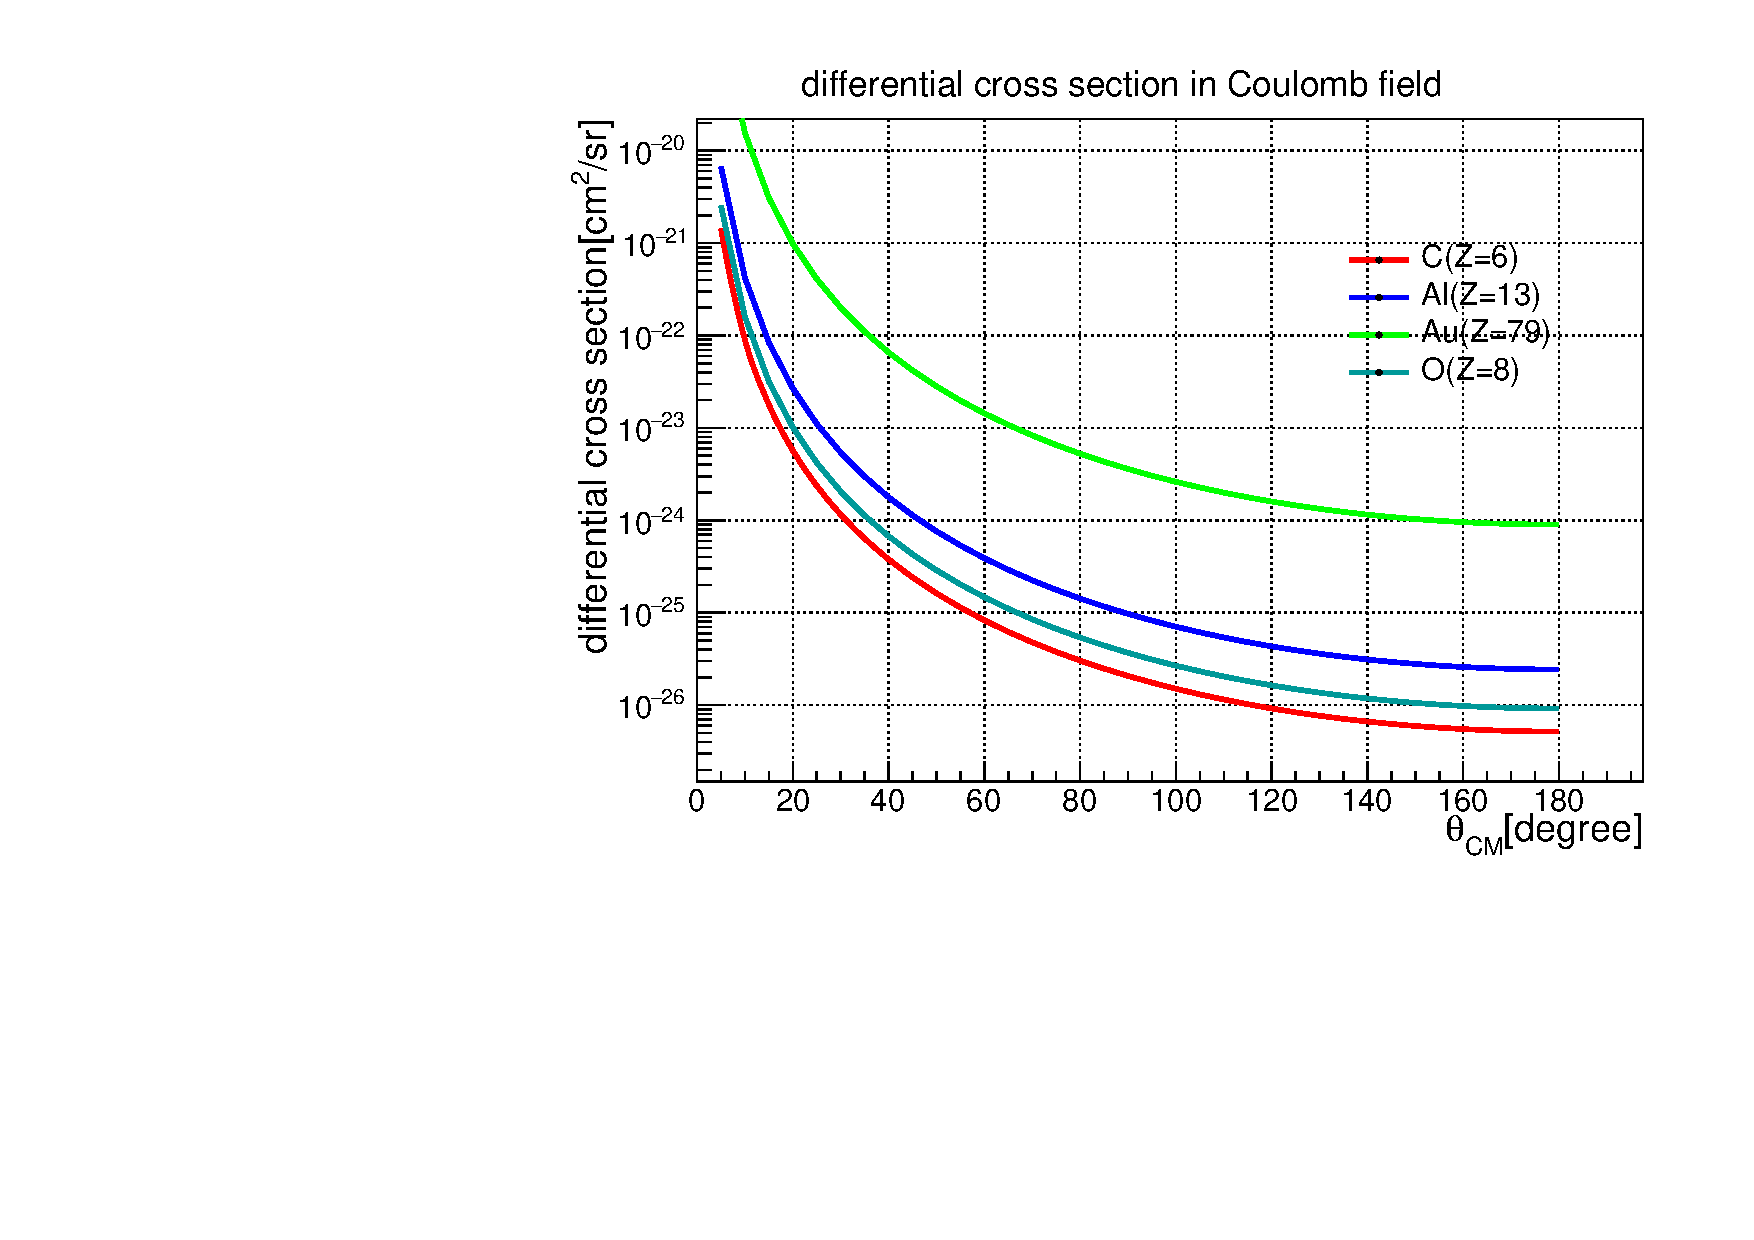
\includegraphics[width=9cm]{picture/cstheory/newcr.pdf}
\caption{クーロン力による微分散乱断面積}
\label{fig:cross}
\end{figure}

\newpage
\subsubsection{同種2粒子系におけるCoulomb散乱\cite{2017}}
以下では、便宜上2つの粒子をそれぞれ粒子1、粒子2と呼称する。

同種粒子の場合、2粒子が異なる場合と比べて以下の2点を修正する必要がある。
\begin{enumerate}
    \item 検出器は粒子1と粒子2を実験的に区別することができないため、断面積$\sigma$を定義し直す必要がある。
    \item 波動関数を定義し直す必要がある。
\end{enumerate}

1つ目については量子力学固有のものではない。p-p散乱では図\ref{fig:ppcm}のような黒と青の2つの経路が考えられる。
今、粒子1の断面積を$\sigma^{(1)}$、粒子2の断面積を$\sigma^{(2)}$とすると、検出器における断面積はそれらの和で書けるため、
\begin{equation*}
    \sigma=\sigma^{(1)}+\sigma^{(2)}
\end{equation*}
と定義できる。ここで$\sigma^{(1)}$は散乱振幅$f(\theta)$を使って、
\begin{equation*}
    \sigma^{(1)}=|f(\theta)|^{2}
\end{equation*}
と表されるとすると、粒子2のほうは重心系で考えているため、
\begin{equation*}
    \sigma^{(2)}=|f(\pi-\theta)|^{2}
\end{equation*}
と表される。
\begin{figure}[htbp]
\centering
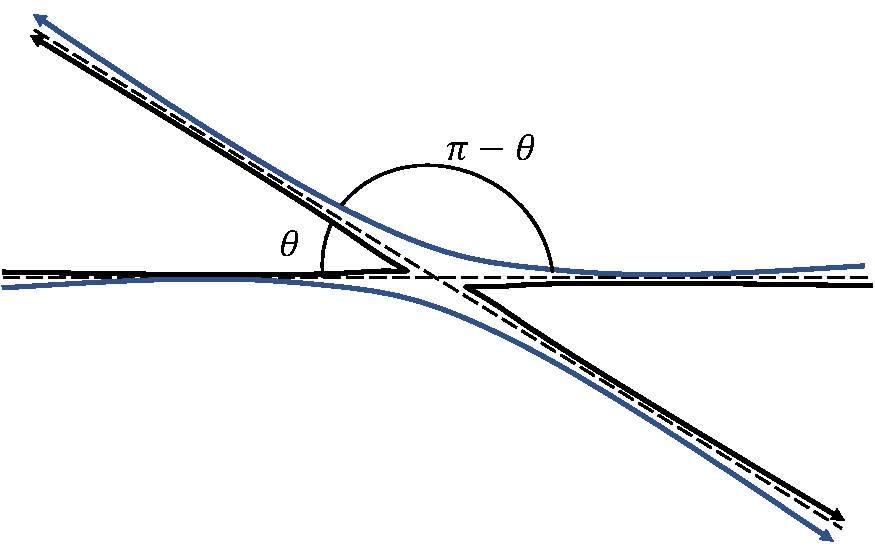
\includegraphics[width=7cm]{picture/cstheory/p-pCM.pdf}
\caption{重心系におけるp-p散乱}
\label{fig:ppcm}
\end{figure}

2つ目については量子力学固有のものである。以下の議論で「対称化する」とは、ボゾンなら完全対称に、フェルミオンなら反対称にすることである。修正前の波動関数の漸近形は\eqref{eq:zenkinn}の形で与えられたが、第一項を$\Psi_{i}$、第二項を$\Psi_{d}$とすると、対称化した波動関数$\Psi'$は
\begin{equation*}
    \Psi'=\Psi_{i}\pm\Psi'_{i}+\Psi_{d}\pm\Psi'_{d}
\end{equation*}
と表せる。$\pm$は$+$がボゾン、$-$がフェルミオンである。ただし、
\begin{align*}
    \Psi'_{i}(\theta)\sim \Psi_{i}(\pi-\theta) \\
    \Psi'_{d}(\theta)\sim \Psi_{d}(\pi-\theta)
\end{align*}
である。よって、$\Psi'$は以下のように表すことができる。
\begin{equation}
    \Psi' \sim \exp(ikz) \pm \exp(-ikz)+f'(\theta)\frac{\exp(ikr)}{r} 
\end{equation}
ただし、
\begin{equation*}
    f'(\theta)=f(\theta)+f(\pi-\theta)
\end{equation*}
であり、対称化振幅と呼ばれる。これで2つの修正ができたことになる。よって、微分散乱断面積は
\begin{equation*}
    \frac{d\sigma}{d\Omega}=|f'(\theta)|^{2}=|f(\theta)+f(\pi-\theta)|^{2}
\end{equation*}
となる。

しかし、今回考える陽子はスピン$\tfrac{1}{2}$を持つのでそのことも考慮しなくてはいけない。そのため、まず一般的にスピンが$s$の同種2粒子の散乱を考える。2粒子の合成スピンの状態の波は全部で\((2s+1)^2\)個あり、1重項状態が1個、3重項状態が3個、$\cdots$、$(4s+1)$重項状態が$(4s+1)$個となっている。$(4t+1)$重項状態に対応する散乱振幅を$f_{4t+1}(\theta)$で表す。
(ただし、$t=0,\tfrac{1}{2},1,\tfrac{3}{2},\cdots,s$) \\*
$t$が整数の時、$(4t+1)$重項に対応する微分散乱断面積は
\begin{equation*}
    \frac{d\sigma}{d\Omega_{4t+1}}=|f_{4t+1}(\theta)+f_{4t+1}(\pi-\theta)|^2
\end{equation*}
であり、$t$が半整数の時、$(4t+1)$重項に対応する微分散乱断面積は
\begin{equation*}
    \frac{d\sigma}{d\Omega_{4t+1}}=|f_{4t+1}(\theta)-f_{4t+1}(\pi-\theta)|^2
\end{equation*}
と表される。

偏りのない粒子同士の衝突において、入射粒子と標的粒子のスピンの方向は偶然に決められるので、微分散乱断面積の計算は重みをつけて考える。だから、
\begin{align}
    \frac{d\sigma}{d\Omega} &= \frac{1}{(2s+1)^{2}}[|f_{1}(\theta)+f_{1}(\pi-\theta)|^{2}+3\,|f_{3}(\theta)-f_{3}(\pi-\theta)|^{2} \notag\\
    &+ \cdots +(4s+1)\,|f_{4s+1}(\theta)+(-1)^{2s}f_{4s+1}(\pi-\theta)|^{2}]\label{eq:spin}
\end{align}
今、クーロン散乱のみを考えているため、散乱振幅にスピンは無関係で、
\begin{equation}
    f_{4t+1}(\theta)=f(\theta) \ \ (t=0,\frac{1}{2},1,\frac{3}{2},\cdots,s)\label{eq:mukankei}
\end{equation}
とできる。

よって、式\eqref{eq:spin}と式\eqref{eq:mukankei}より、
\begin{align}
     \frac{d\sigma}{d\Omega} &= \frac{1}{(2s+1)^{2}}[|f_{1}(\theta)+f_{1}(\pi-\theta)|^{2}+3\,|f_{3}(\theta)-f_{3}(\pi-\theta)|^{2} \notag\\
    &+ \cdots +(4s+1)\,|f_{4s+1}(\theta)+(-1)^{2s}f_{4s+1}(\pi-\theta)|^{2}] \notag\\
 &= |f(\theta)|^2+|f(\pi-\theta)|^2\notag\\
     &+\frac{1}{(2s+1)^{2}}[1-3+5-\cdots+(-1)^{2s}(4s+1)][f(\theta)f^*(\pi-\theta)+f^*(\theta)f(\pi-\theta)] \notag\\
 &= |f(\theta)|^2+|f(\pi-\theta)|^2\notag\\
   &+\frac{1}{(2s+1)^{2}}\,2\,(-1)^{2s}(2s+1)[f(\theta)f^*(\pi-\theta)+f^*(\theta)f(\pi-\theta)] \notag\\
    &= |f(\theta)|^2+|f(\pi-\theta)|^2 +(-1)^{2s}\frac{2}{(2s+1)}[f(\theta)f^*(\pi-\theta)+f^*(\theta)f(\pi-\theta)] 
\end{align}
これに散乱振幅$f(\theta)$の式\eqref{eq:sanransinpuku}を代入すると、
\begin{equation}
   \frac{d\sigma}{d\Omega} = \left(\frac{Z_{1}Z_{2}e^2}{16\pi\varepsilon_{0}E}\right)^{2}\left[\frac{1}{\sin^4\frac{\theta}{2}}+\frac{1}{\cos^4\frac{\theta}{2}}+(-1)^{2s}\frac{2}{2s+1}\frac{\cos[\frac{Z_{1}Z_{2}e^2}{4\pi\varepsilon_{0}\hbar v}\ln(\tan^2\frac{\theta}{2})]}{\sin^2\frac{\theta}{2}\cos^2\frac{\theta}{2}}\right]
   \label{eq:dousyucs}
\end{equation}
今回はp-p散乱(陽子-陽子散乱)なので、$Z_{1}=Z_{2}=1,s=\frac{1}{2}$を\eqref{eq:dousyucs}に代入すると、
\begin{equation}
   \frac{d\sigma}{d\Omega} = \left(\frac{e^2}{16\pi\varepsilon_{0}E}\right)^{2}\left[\frac{1}{\sin^4\frac{\theta}{2}}+\frac{1}{\cos^4\frac{\theta}{2}}-\frac{\cos[\frac{e^2}{4\pi\varepsilon_{0}\hbar v}\ln(\tan^2\frac{\theta}{2})]}{\sin^2\frac{\theta}{2}\cos^2\frac{\theta}{2}}\right]
   \label{eq:Mott}
\end{equation}
となる。式\eqref{eq:Mott}をMottの散乱公式という。

本実験では$E=$\;3\;MeVなので、この場合の式\eqref{eq:Mott}のグラフは図\ref{fig:Mott}のようになる。図\ref{fig:Mott}より、微分散乱断面積は散乱角$90^{\circ}$を境に対称的な形をとることがわかる。
\begin{figure}[htbp]
\centering
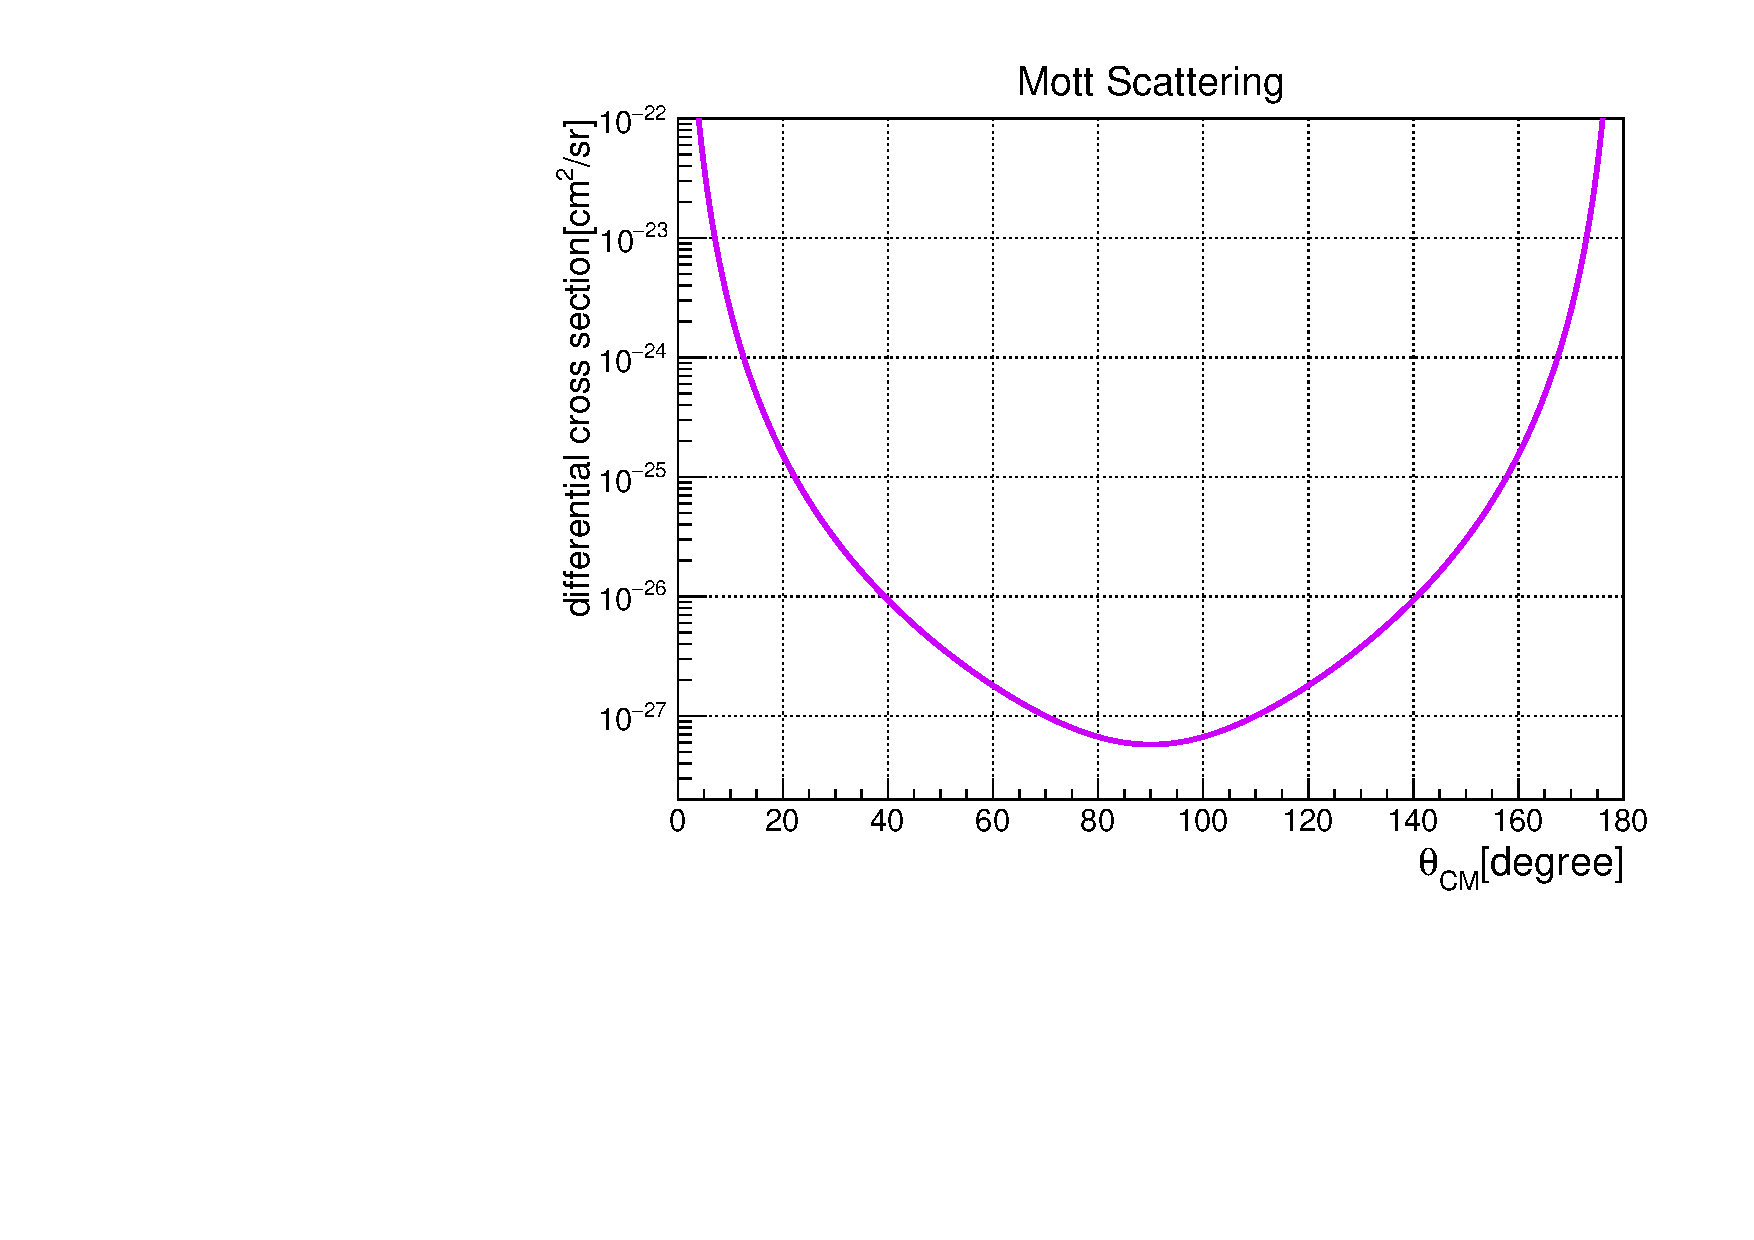
\includegraphics[width=9cm]{picture/cstheory/Mott_revise.pdf}
\caption{Mott散乱による微分散乱断面積}
\label{fig:Mott}
\end{figure}

\newpage
\subsubsection{核力による散乱}\label{NF}
加速された陽子が標的となる試料に入射したときに散乱される要因として、核力による散乱も考えられる。ここでは古典的に、陽子と標的原子核の衝突を剛体球による散乱と近似し、剛体球による微分断面積を考える。

\begin{figure}[htbp]
\centering
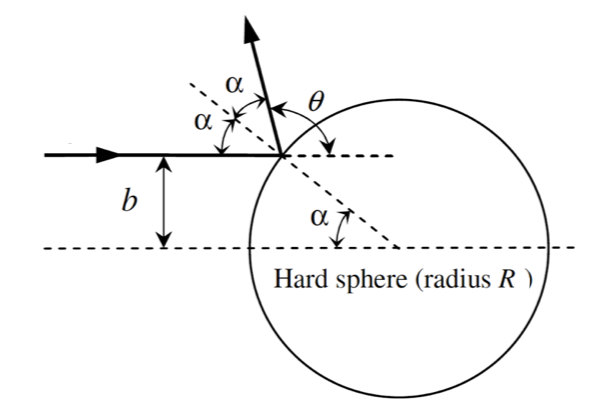
\includegraphics[width=7cm]{picture/cstheory/NF.png}
\caption{剛体球による散乱の様子(\cite{ion}より引用し、一部改変)}
\label{fig:NF}
\end{figure}

図\ref{fig:NF}のような状況を考える。この場合の微分散乱断面積は、全立体角$4\pi$に対して陽子から見た球のシルエットの面積の比をとればよく、その面積は$\pi R^{2}$なので、 \\
求める微分散乱断面積は、
\begin{equation}
    \frac{d\sigma}{d\Omega}=\frac{R^{2}}{4}
    \label{eq:nfcr1}
\end{equation}
となる。

陽子半径$r$を考慮する場合は、\eqref{eq:nfcr1}右辺の$R$を$R+r$に書き換えればよく\cite{ion}、この場合の剛体球による微分散乱断面積は、
\begin{equation}
    \frac{d\sigma}{d\Omega}=\frac{(R+r)^{2}}{4}
    \label{eq:nfcr2}
\end{equation}
と表される。

本研究では、核力による散乱を式\eqref{eq:nfcr2}で表される剛体球による散乱として解析を行う。



\end{document}